\chapter{Beschreibung der verschiedenen Messungen und Ergebnisdarstellung}

\section{Initial Setup eines Switch}\label{switch}

Zun�chst wird der Cisco 2960 Switch, mittels einem RJ-45-to-DB-9 connector
console Kabel, an einen Computer angeschlossen.\\Nach der Verkabelung wird
HyperTerminal, das genutzte Terminal-Emulations-Programm auf dem Computer
gestartet.
\newline
Der genutzte Port, in diesem Fall COM1, wird ausge�hlt und die Parameter f�r die
Terminal Emulation werden nach den Vorgaben des Versuchs konfiguriert. Nach
diesen Einstellungen wird erst der Switch gestartet.
\newline
Um den Switch neu initialisieren zu k�nnen, m�ssen erst die bereits vorhandenen
Konfigurationen gel�scht werden. Dies geschieht �ber den ``privilledged EXEC
mode'' (enable)\footnote{In diesem Dokument werden die genutzten Kommandos
\textit{kursiv} dargestellt.}\\
\newline
\underline{Vorgehensweise:}
\begin{itemize}
  \item \acs{VLAN}-Datei l�schen (\textit{delete flash:vlan.dat})
  \item Startup-Config-Datei l�schen (\textit{erase startup-config})
  \item Software neustarten (\textit{reload})
\end{itemize}



\section{Initial Setup eines Routers}

�quivalent zum Initial Setup des Switchs in \ref{switch} wird der Cisco
2811 Router mit einem Computer verbunden, das Programm HyperTerminal gestartet
und die Konfigurationen des Emulations-Programms, wie im Versuch beschrieben,
vorgenommen. Nach diesen Schritten wird der Router gestartet.

\clearpage

\section{Informationen des Router Systems}

Durch \textit{show running-config} im Priviledged Mode werden die aktuellen
Router-Konfigurationen im RAM angezeigt.\\Danach wird der Configuration Mode
(\textit{configure terminal}) genutzt um �nderungen vorzunehmen. In der
aktuellen Konfiguration lautet der Hostname ``Router''. Dieser wird nun mittels
\textit{hostname} in ``R1\textunderscore HTW'' ge�ndert.
\newline
Ein erneutes Ausgeben der running-config zeigt, dass der Hostname erfolgreich
ge�ndert wurde.

\subsection{Startup-Config}
Mittels \textit{show startup-config} soll die entsprechende Konfigurationsdatei
angezeigt werden. Nach Eingabe des Kommandos ist zu erkennen, dass solch eine
Datei nicht existiert.
\newline
Die vorgenommene �nderung wird nur in der Running-Config gespeichert, nicht in
der Startup-Config. Durch Kopieren der Running- in die
Startup-Konfiguratiosdatei sind die �nderungen beim n�chsten Bootvorgang des
Routers verf�gbar.\\
\newline
\underline{Vorgehensweise:}
\begin{itemize}
  \item �berschreiben der Startup-Config (\textit{copy running-config
  startup-config})
  \item Neustart des Routers (\textit{reload})
\end{itemize}

Da der Router nach dem Neustart den Hostnamen ``R1\textunderscore HTW'' anzeigt,
hat das �berschreiben der Startup-Config funktioniert.

\subsection{Router zur�cksetzen}

Um die Default-Einstellungen wiederherzustellen wird im Priviledged Mode die
Startup-Config gel�scht (\textit{erase startup-config}). Um den Vorgang
abzuschlie�en wird der Router neugestartet (\textit{reload}).

\clearpage

\section{Packet Tracer}

\subsection{Versuchsaufbau}
F�r eine Einf�hrung in die Software ``Packet Tracer'' wird folgender Aufbau
erstellt:
\begin{figure}[h!]
\centering
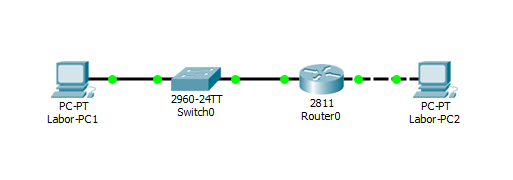
\includegraphics[width=\textwidth]{Graphics/PacketTracer.PNG}
\caption{Versuchsaufbau im Packet Tracer}
\label{fig:ping}
\end{figure}

\subsection{Konfiguration}
Die Ger�te des Versuchaufbaus werden wie folgt konfiguriert:


\begin{table}[!htbp]
\centering
\small
	\begin{tabularx}{1.05\textwidth}{|X|X|X|X|X|X|}
	\hline
	\textbf{Device} & \textbf{Hostname} & \textbf{Interface} & \textbf{IP-Address} &
	\textbf{Subnet Mask} & \textbf{Default \newline Gateway} \\
	\hline
	PC0 	& Labor-PC1		& Fast-Ethernet	& 192.168.0.10 	& 255.255.255.128 &
	192.168.0.1
	\\
	\hline
	Switch0 & Labor-Switch1 & FE0/0 \newline FE0/1 & NA		& NA			& NA \\
	\hline
	Router0 & Labor-Router1 & FE0/0 \newline FE0/1 & 192.168.0.1 \newline 10.10.10.1
	& 255.255.255.128 \newline 255.255.255.224 & NA \newline NA \\
	\hline
	PC1 	& Labor-PC2 	& Fast-Ethernet & 10.10.10.10	& 255.255.255.224	& 10.10.10.1
	\\
	\hline
	\end{tabularx}
\caption{Konfiguration der Ger�te im Packet Tracer}
\label{config}
\end{table}

\clearpage

\subsection{Konnektivit�t �berpr�fen}
Die Konnektivit�t wird im ``Realtime Modus'' des Packet Tracers �berpr�ft.
Hierzu werden Ping-Befehle verwendet.
\begin{itemize}
  \item Ping von PC1 zu Router1, FE0/0
  \newline
\begin{lstlisting}
PC>ping 192.168.0.1

Pinging 192.168.0.1 with 32 bytes of data:

Reply from 192.168.0.1: bytes=32 time=62ms TTL=255
Reply from 192.168.0.1: bytes=32 time=62ms TTL=255
Reply from 192.168.0.1: bytes=32 time=62ms TTL=255
Reply from 192.168.0.1: bytes=32 time=63ms TTL=255

Ping statistics for 192.168.0.1:
    Packets: Sent = 4, Received = 4, Lost = 0 (0% loss),
Approximate round trip times in milli-seconds:
    Minimum = 62ms, Maximum = 63ms, Average = 62ms
  \end{lstlisting}
  \item Ping von PC1 zu Router1, FE0/1
  \newline
\begin{lstlisting}
PC>ping 10.10.10.1

Pinging 10.10.10.1 with 32 bytes of data:

Reply from 10.10.10.1: bytes=32 time=62ms TTL=255
Reply from 10.10.10.1: bytes=32 time=62ms TTL=255
Reply from 10.10.10.1: bytes=32 time=47ms TTL=255
Reply from 10.10.10.1: bytes=32 time=49ms TTL=255

Ping statistics for 10.10.10.1:
    Packets: Sent = 4, Received = 4, Lost = 0 (0% loss),
Approximate round trip times in milli-seconds:
    Minimum = 47ms, Maximum = 62ms, Average = 55ms
\end{lstlisting}
  \item Ping von PC2 zu Router1, FE0/1
  \newline
\begin{lstlisting}

PC>ping 10.10.10.1

Pinging 10.10.10.1 with 32 bytes of data:

Reply from 10.10.10.1: bytes=32 time=31ms TTL=255
Reply from 10.10.10.1: bytes=32 time=31ms TTL=255
Reply from 10.10.10.1: bytes=32 time=32ms TTL=255
Reply from 10.10.10.1: bytes=32 time=32ms TTL=255

Ping statistics for 10.10.10.1:
    Packets: Sent = 4, Received = 4, Lost = 0 (0% loss),
Approximate round trip times in milli-seconds:
    Minimum = 31ms, Maximum = 32ms, Average = 31ms

\end{lstlisting}  
  \item Ping von PC2 zu PC1
  \newline
\begin{lstlisting}
PC>ping 192.168.0.10

Pinging 192.168.0.10 with 32 bytes of data:

Reply from 192.168.0.10: bytes=32 time=93ms TTL=127
Reply from 192.168.0.10: bytes=32 time=94ms TTL=127
Reply from 192.168.0.10: bytes=32 time=94ms TTL=127
Reply from 192.168.0.10: bytes=32 time=109ms TTL=127

Ping statistics for 192.168.0.10:
    Packets: Sent = 4, Received = 4, Lost = 0 (0% loss),
Approximate round trip times in milli-seconds:
    Minimum = 93ms, Maximum = 109ms, Average = 97ms
\end{lstlisting}
\end{itemize}

Der ping-Test zeigt, dass alle Ger�te erreichbar und korrekt konfiguriert sind.

\clearpage

\subsection{Simulation eines Echo Request/Echo Reply}

F�r diesen Teil des Versuchs wird der ``Simulation Mode'' des Packet Tracers
verwendet. PC1 stellt die Quelle, und der Router das Ziel, dar. Es werden nur
\acs{ICMP} Pakete f�r die �bertragung gefiltert.

\subsubsection{Analyse eines Ping Befehls}

Die folgenden Diagramme \ref{fig:ping} und \ref{fig:pong} veranschaulichen auf
welchen Schichten Switch und Router im \acs{ISO}-\acs{OSI}-Referenzmodell
arbeiten.

\begin{figure}[h!]
\centering
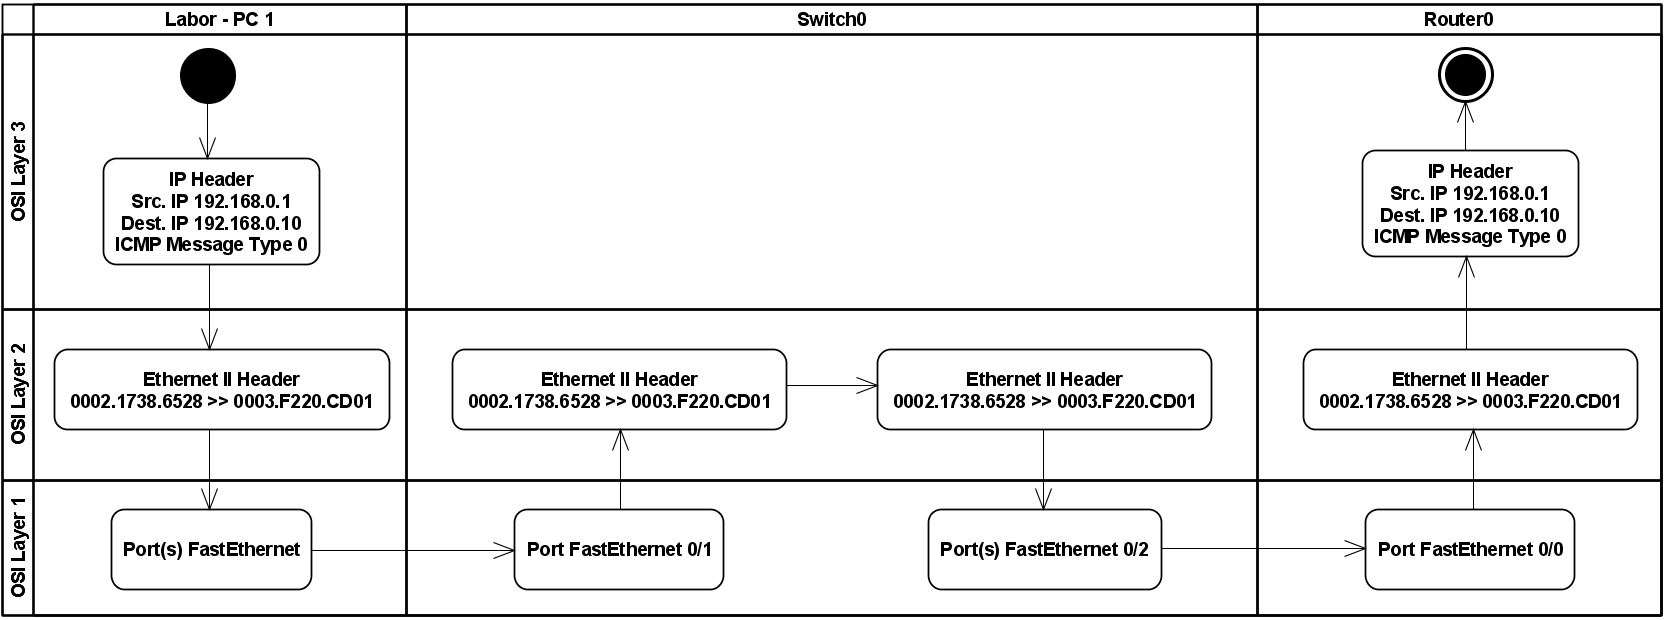
\includegraphics[scale=0.37]{Graphics/PcToRouter.PNG}
\caption{Echo Request von PC1 zum Router}
\label{fig:ping}
\end{figure}

Hier (\ref{fig:ping}) dargestellt ist der Echo Request (ICMP Message Type 8) vom
Labor-PC1 zum Router. Den Ethernet-Headern sind die \acs{MAC}-Adressen der
Quelle und des Ziels zu entnehmen.\\Es handelt sich um einen Layer-2-Switch in diesem
Versuchsaufbau.

\begin{figure}[h!]
\centering
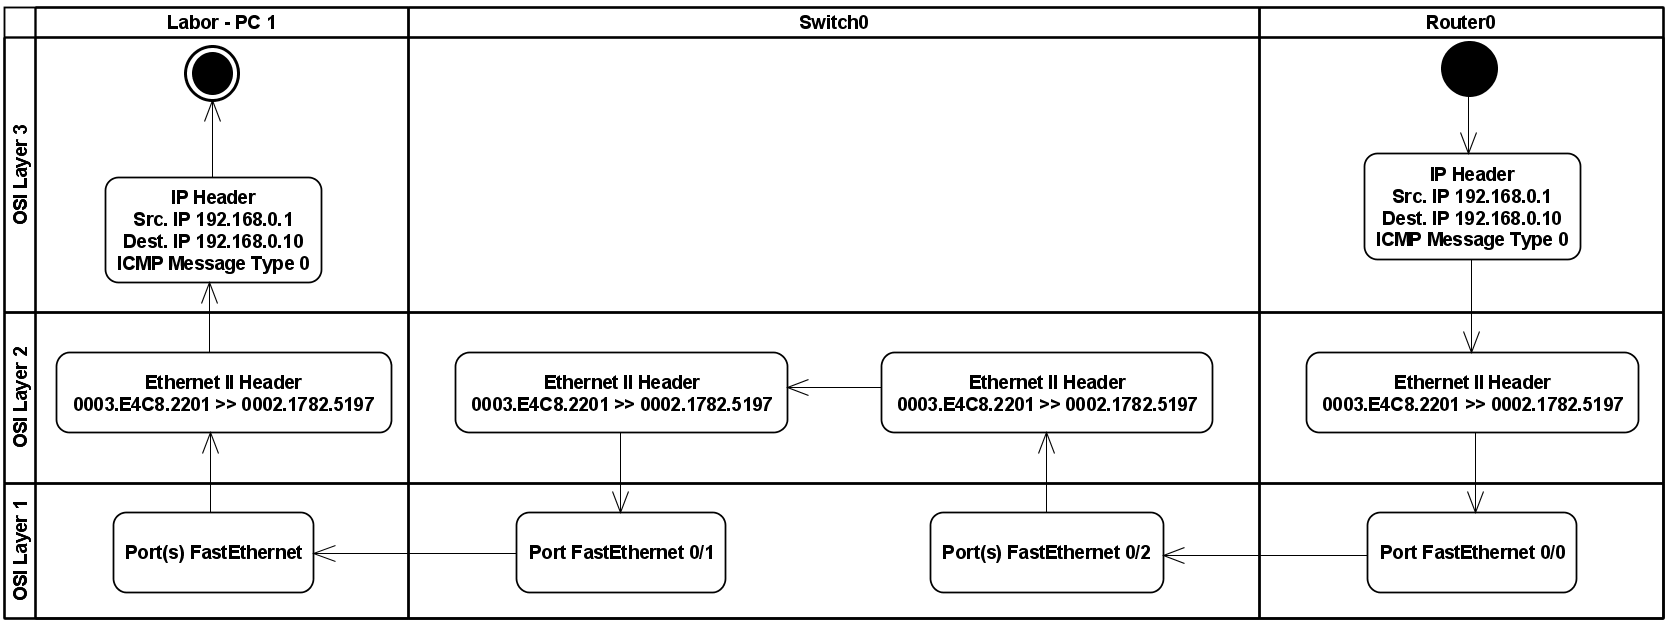
\includegraphics[scale=0.37]{Graphics/RouterToPc.PNG}
\caption{Echo Reply vom Router zum PC1}
\label{fig:pong}
\end{figure}

�quivalent zum Echo Request ist in \ref{fig:pong} der Echo Reply (ICMP Message
Type 0) vom Router zum Labor-PC1 dargestellt.
